% -*- mode: latex; -*- mustache tags:  
\documentclass[10pt,twoside,english]{_support/latex/sbabook/sbabook}
\let\wholebook=\relax

\usepackage{import}
\subimport{_support/latex/}{common.tex}

%=================================================================
% Debug packages for page layout and overfull lines
% Remove the showtrims document option before printing
\ifshowtrims
  \usepackage{showframe}
  \usepackage[color=magenta,width=5mm]{_support/latex/overcolored}
\fi


% =================================================================
\title{A PharoThings Tutorial}
\author{Allex Oliveira}
\series{Square Bracket tutorials}

\hypersetup{
  pdftitle = {A PharoThings Tutorial},
  pdfauthor = {Allex Oliveira},
  pdfkeywords = {IoT, Raspberry, PharoThings, Pharo}
}


% =================================================================
\begin{document}

% Title page and colophon on verso
\maketitle
\pagestyle{titlingpage}
\thispagestyle{titlingpage} % \pagestyle does not work on the first one…

\cleartoverso
{\small

  Copyright 2017 by Allex Oliveira.

  The contents of this book are protected under the Creative Commons
  Attribution-ShareAlike 3.0 Unported license.

  You are \textbf{free}:
  \begin{itemize}
  \item to \textbf{Share}: to copy, distribute and transmit the work,
  \item to \textbf{Remix}: to adapt the work,
  \end{itemize}

  Under the following conditions:
  \begin{description}
  \item[Attribution.] You must attribute the work in the manner specified by the
    author or licensor (but not in any way that suggests that they endorse you
    or your use of the work).
  \item[Share Alike.] If you alter, transform, or build upon this work, you may
    distribute the resulting work only under the same, similar or a compatible
    license.
  \end{description}

  For any reuse or distribution, you must make clear to others the
  license terms of this work. The best way to do this is with a link to
  this web page: \\
  \url{http://creativecommons.org/licenses/by-sa/3.0/}

  Any of the above conditions can be waived if you get permission from
  the copyright holder. Nothing in this license impairs or restricts the
  author's moral rights.

  \begin{center}
    
\includegraphics[width=0.2\textwidth]{_support/latex/sbabook/CreativeCommons-BY-SA.pdf}
  \end{center}

  Your fair dealing and other rights are in no way affected by the
  above. This is a human-readable summary of the Legal Code (the full
  license): \\
  \url{http://creativecommons.org/licenses/by-sa/3.0/legalcode}

  \vfill

  % Publication info would go here (publisher, ISBN, cover design…)
  Layout and typography based on the \textcode{sbabook} \LaTeX{} class by Damien
  Pollet.
}


\frontmatter
\pagestyle{plain}

\tableofcontents*
\clearpage\listoffigures

\mainmatter

\chapter{Installations }
The first step you need to get started with PharoThings is to install an Operating System in your Raspberry Pi. When you buy a Raspberry Pi, the OS is not factory installed.
\section{Installating OS on RASPBERRY (RASPBIAN)}
In this chapter, we will download and install NOOBS (New Out Of the Box Software). NOOBS is an easy operating system installer which contains Raspbian (\url{https://www.raspberrypi.org/downloads/raspbian/}) and LibreELEC (\url{https://libreelec.tv}).

Raspbian is the Foundation’s official supported operating system, a Linux OS based on Debian Stretch to run in ARM processors.
\subsection{Download}
You can download an official image from the Raspberry Pi website Noobs downloads page (\url{https://www.raspberrypi.org/downloads/noobs/}). You will download a zip file and extract the files to your SD card.
\subsection{Copying}
You will need a computer with an SD card reader to install the image.
This process basically extracts the files from the zip file downloaded into an SD card formatted and start the Raspberry Pi with this SD card.

You can go directly to your operating system by clicking on the links below:
\section{Copying Raspbian files on MAC OSX}
\begin{itemize}
\item Open “disk utility”, select the SD Card and Erase (Format MS-DOS FAT) as shown in Figure \ref{macInstall}.
\end{itemize}

\begin{itemize}
\item Copy the files from folder NOOBS\_xxx to SD Card as shown in Figure \ref{macCopy}.
\end{itemize}


\begin{figure}

\begin{center}
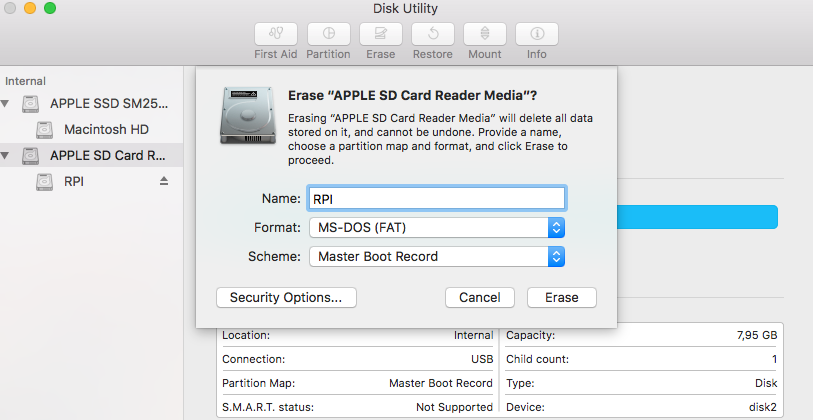
\includegraphics[width=0.7\textwidth]{/Users/allexoliveira/PharoThingsBook/Booklet-APharoThingTutorial/_result/pdf/Chapters/Chap1GettingStarted/figures/pharothings-install-raspberry-pi-raspbian-osx-arm.png}\caption{Preparing SD Card.\label{macInstall}}\end{center}
\end{figure}



\begin{figure}

\begin{center}
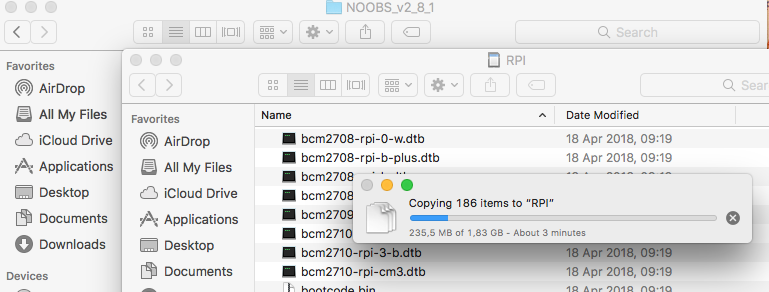
\includegraphics[width=0.7\textwidth]{/Users/allexoliveira/PharoThingsBook/Booklet-APharoThingTutorial/_result/pdf/Chapters/Chap1GettingStarted/figures/pharothings-install-raspberry-pi-raspbian-linux-arm-copy.png}\caption{Copying NOOBS.\label{macCopy}}\end{center}
\end{figure}

\section{Copying Raspbian files on Linux}\section{Copying Raspbian files on Windows}\section{Installing the Raspbian in Raspberry Pi}
Insert the SD Card on Raspberry and turn it on. Select “Raspbian” and “Yes” as shown by Figure \ref{install}.


\begin{figure}

\begin{center}
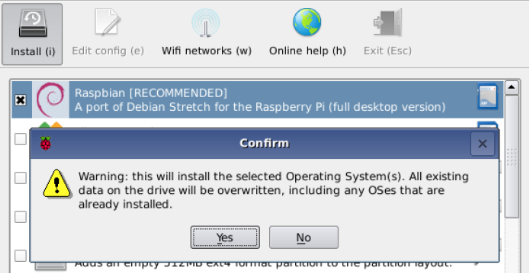
\includegraphics[width=0.6\textwidth]{/Users/allexoliveira/PharoThingsBook/Booklet-APharoThingTutorial/_result/pdf/Chapters/Chap1GettingStarted/figures/pharothings-install-raspberry-pi-raspbian-linux-arm-install.png}\caption{Installing Raspbian.\label{install}}\end{center}
\end{figure}


In a few minutes, you will have your Raspberry Pi running Raspbian OS.
Now you can install PharoThings and control devices remotely. 
\section{Installing PharoThings on Raspberry Pi}
Install PharoThings requires to get Pharo, PharoThings and an ARM virtual machine. 
\subsection{Download PharoLauncher}
Use the PharoLauncher (an application to help you running multiple versions and images of Pharo) and install Pharo 6.1. You can get the launcher from \url{http://pharo.org/download}.
You can also directly install a version of Pharo from the same place.


\begin{figure}

\begin{center}
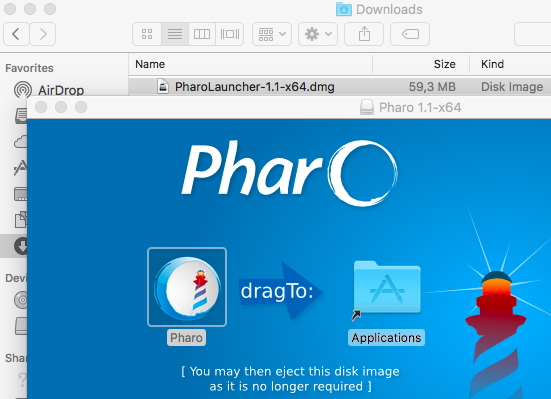
\includegraphics[width=0.6\textwidth]{/Users/allexoliveira/PharoThingsBook/Booklet-APharoThingTutorial/_result/pdf/Chapters/Chap1GettingStarted/figures/InstallLauncher.png}\caption{Installing PharoLauncher.\label{installLauncher}}\end{center}
\end{figure}

\subsection{Download Pharo 61}
Run the Pharo Launcher. Double click the distribution you want to create a image and give a name to image (see Figure \ref{InstallPharo61}). A short name and without spaces is recommended, because we will type this name and path in command line on Linux. 


\begin{figure}

\begin{center}
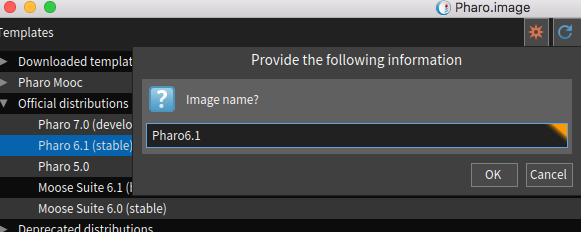
\includegraphics[width=0.6\textwidth]{/Users/allexoliveira/PharoThingsBook/Booklet-APharoThingTutorial/_result/pdf/Chapters/Chap1GettingStarted/figures/Select61.png}\caption{Download Pharo 61.\label{InstallPharo61}}\end{center}
\end{figure}

\subsection{Execute your Pharo image}
Launch the image as shown in Figure \ref{Execute61}. A folder with the image name will be created inside the folder Pharo:  \textcode{/Users/your\_user\_name/Documents/Pharo/}

In this example the folder is  \textcode{/Users/my\_user\_name/Documents/Pharo/Pharo6.1}


\begin{figure}

\begin{center}
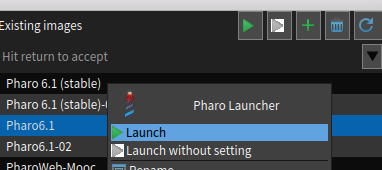
\includegraphics[width=0.6\textwidth]{/Users/allexoliveira/PharoThingsBook/Booklet-APharoThingTutorial/_result/pdf/Chapters/Chap1GettingStarted/figures/Execute61.png}\caption{Open your Pharo image.\label{Execute61}}\end{center}
\end{figure}

\subsection{Load PharoThings}
Open Playground and execute this command to install the server part of PharoThings (as shown in Figure \ref{LoadingPharoThings}):

\begin{displaycode}{plain}
Metacello new
	baseline: 'PharoThings';
	repository: 'github://pharo-iot/PharoThings/src';
	load: #(RemoteDevServer Raspberry).
\end{displaycode}


\begin{figure}

\begin{center}
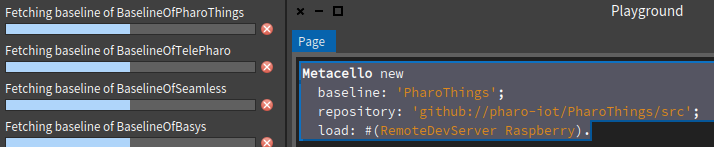
\includegraphics[width=0.6\textwidth]{/Users/allexoliveira/PharoThingsBook/Booklet-APharoThingTutorial/_result/pdf/Chapters/Chap1GettingStarted/figures/LoadingPharoThings.png}\caption{Loading PharoThings.\label{LoadingPharoThings}}\end{center}
\end{figure}


Then configure image to disable slow browser plugins (instead remote browser will be much slower):

\begin{displaycode}{plain}
ClySystemEnvironmentPlugin disableSlowPlugins.
\end{displaycode}
\subsection{Snapshot your Image}
 In Pharo, click and “Save and Quit”. This way all your code and configurations are saved and ready to be reused.
 
 
\subsection{Download the VM}
\begin{itemize}
\item Download ArmVM from \url{http://files.pharo.org/vm/pharo-spur32/linux/armv6/latest.zip}.
\item Unzip it
\item Copy the files shown in FIgure \ref{CopyARM}  to Pharo folder \textcode{/Users/your\_user\_name/Documents/Pharo/pharo\_image\_folder} 
\end{itemize}


\begin{figure}

\begin{center}
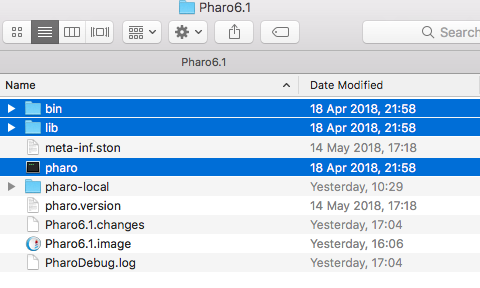
\includegraphics[width=0.6\textwidth]{/Users/allexoliveira/PharoThingsBook/Booklet-APharoThingTutorial/_result/pdf/Chapters/Chap1GettingStarted/figures/CopyARM.png}\caption{Copying PharoARM.\label{CopyARM}}\end{center}
\end{figure}

\subsection{Copying Sources}
Copy the file PharoV60.sources from the folder \textcode{/Applications/Pharo.app/Contents/MacOS} to folder \textcode{/Users/your\_user\_name/Documents/Pharo/images/pharo\_image\_folder/lib/pharo/5.0-201804182009/}
\subsection{Copy to the Raspberry}
Copy this folder to your Raspberry Pi (via flashdrive, network etc). The folder must have the structure shown in Figure \ref{OnRasp}.


\begin{figure}

\begin{center}
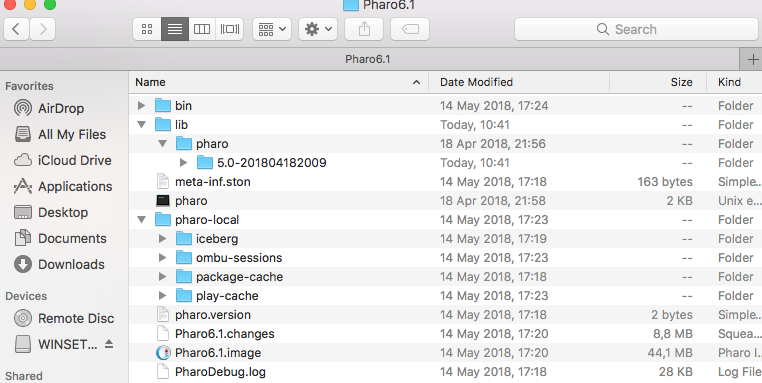
\includegraphics[width=0.6\textwidth]{/Users/allexoliveira/PharoThingsBook/Booklet-APharoThingTutorial/_result/pdf/Chapters/Chap1GettingStarted/figures/OnRasp.png}\caption{Copying the folder on your Raspberry.\label{OnRasp}}\end{center}
\end{figure}

\section{Execute PharoThings on Raspberry}\subsection{Turn on your Raspberry and connect it to the network.}
In this example, the folder Pharo6.1 was copied to folder \textcode{/home/pi/}.

Is necessary apply execute permissions on the Pharo files, using the command chmod +x

\begin{displaycode}{plain}
chmod +x /home/pi/Pharo6.1/pharo

chmod +x /home/pi/Pharo6.1/lib/pharo/5.0-201804182009/pharo
\end{displaycode}
\subsection{Start Server}
Start the Pharo typing the following command in the Terminal on your Raspberry :

\begin{displaycode}{plain}
pharo --headless Server.image remotePharo --startServerOnPort=40423
\end{displaycode}

If all is right, you will see the answer:

\begin{displaycode}{plain}
'a TlpRemoteUIManager is registered on port 40423'
\end{displaycode}

So now we have the Raspberry running the TelePharo on TCP port 40423 (as shown in Figure \ref{Commandline}) and we can connect into it from another computer.


\begin{figure}

\begin{center}
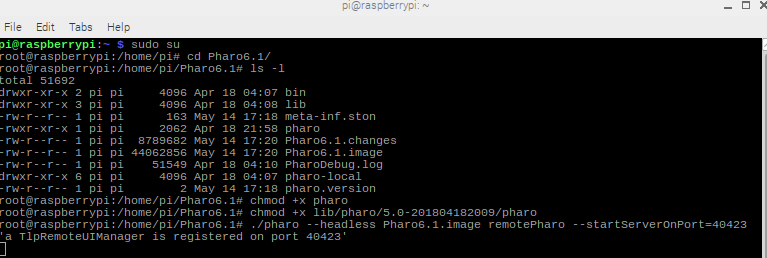
\includegraphics[width=0.6\textwidth]{/Users/allexoliveira/PharoThingsBook/Booklet-APharoThingTutorial/_result/pdf/Chapters/Chap1GettingStarted/figures/Commandline.png}\caption{Server up and running.\label{Commandline}}\end{center}
\end{figure}

\section{Connecting Pharo client on remote Pharo}
Open again the Pharo on your local computer and execute this command to install the PharoThings client:

\begin{displaycode}{plain}
Metacello new
baseline: 'PharoThings';
repository: 'github://pharo-iot/PharoThings/src';
load: 'RemoteDev.
\end{displaycode}

Type this command to connect to the remote TelePharo on Raspberry (change the IP to your Raspberry IP):

\begin{displaycode}{plain}
remotePharo := TlpRemoteIDE connectTo: (TCPAddress ip: #[193 51 236 167] port: 40423)
\end{displaycode}

Here we are using specialized Raspberry tools. They require the auto-refresh feature of inspector which is not enabled by default in Pharo 6. To activate it evaluate:

\begin{displaycode}{plain}
GTInspector enableStepRefresh
\end{displaycode}

So for your board model you need to choose an appropriate board class. For Raspberry, it will be one of the RpiBoard subclasses. Currently, you can use the following classes according to the models:

\begin{itemize}
\item RpiBoardBRev1: Raspberry Pi Model B Revision 1
\item RpiBoardBRev2: Raspberry Pi Model B Revision 2
\item RpiBoard3B: Raspberry Pi Model B+, Pi2 Model B, Pi3 Model B, Pi3 Model B+
\end{itemize}

With the chosen class evaluate the following code to open an inspector:

\begin{displaycode}{plain}
remoteBoard := remotePharo evaluate: [ RpiBoardBRev1 current].
remoteBoard inspect.
\end{displaycode}

And will be open the inspector showing the PIN scheme (as shown in Figure \ref{PharoThingsinspector})


\begin{figure}

\begin{center}
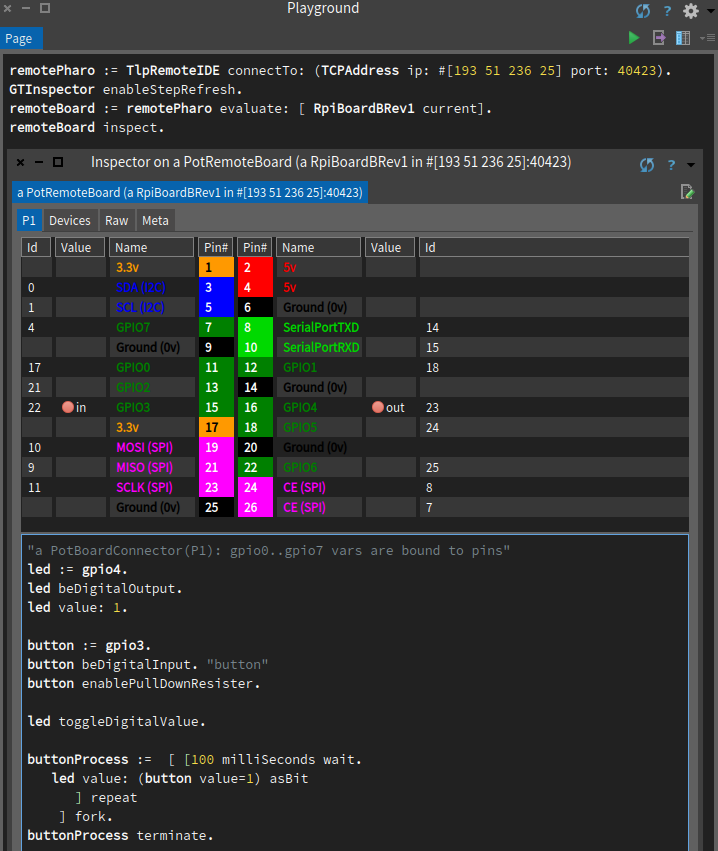
\includegraphics[width=0.6\textwidth]{/Users/allexoliveira/PharoThingsBook/Booklet-APharoThingTutorial/_result/pdf/Chapters/Chap1GettingStarted/figures/PharoThingsInspector.png}\caption{Remote GPIO inspector\label{PharoThingsinspector}}\end{center}
\end{figure}


The board inspector provides a scheme of pins similar to Raspberry Pi docs. But here it is a live tool which represents the current pins state.

In the picture the board is shown with two configured pins: gpio3 and gpio4 which are connected to physical button and led accordingly.

Digital pins are shown with green/red icons which represent high/low (1/0) values. In case of output pins you are able to click on the icon to toggle the value. Icons are updated according to pin value changes. If you click on physical button on your board the inspector will show the updated pin state by changing its icon color.

The evaluation pane in the bottom of the inspector provides bindings to gpio pins which you can script by \#doIt/printIt commands. The example shows expressions which were used to configure a button and led.
\section{In the next chapter}
Now that we have installed the Operation System and PharoThings in the Raspberry Pi, we can play with LEDs, sensors, LCD displays and more. 

In the next chapter we will see how turing on/off a LED using PharoThings. 


% lulu requires an empty page at the end. That's why I'm using
% \backmatter here.
\backmatter

% Index would go here

\end{document}
